\documentclass[aps,prd]{revtex4-1}

\usepackage{hyperref}
\usepackage{amsmath}
\usepackage{amssymb}
\usepackage{graphicx}
\usepackage{color}

\newcommand{\order}[1]{\mathcal{O}\left( #1 \right)}
\newcommand{\fixme}[1]{\textbf{FIXME: #1}}
\newcommand{\mathset}[1]{\left\{ #1 \right\}}

\newcommand{\xmin}{x_\mathrm{min}}

\newcommand{\ilya}[1]{{\color{red} \bf #1}}
\newcommand{\will}[1]{{\color{blue} \bf #1}}
\newcommand{\jon}[1]{{\color{orange} \bf  #1}}

\DeclareMathOperator{\erf}{erf}

\begin{document}

\title{Bayesian Rate Estimation}

\author{Will M. Farr}
\email{w-farr@northwestern.edu}
\homepage{http://faculty.wcas.northwestern.edu/will-farr/}
\affiliation{Center for Interdisciplinary Exploration and Research in Astrophysics\\
Department of Physics and Astronomy\\
Northwestern University, 2145 Sheridan Road, Evanston, IL 60208}
%\affiliation{Northwestern University and CIERA}

\author{Ilya Mandel}
\email{imandel@star.sr.bham.ac.uk}
\homepage{http://www.sr.bham.ac.uk/~imandel}
\affiliation{School of Physics and Astronomy\\University of Birmingham\\Edgbaston B15 2TT Birmingham\\United Kingdom}
%\affiliation{University of Birmingham}

\author{Jonathan R. Gair}
\email{jrg23@cam.ac.uk}

\begin{abstract}
  We show how to obtain a Bayesian estimate of the rate of signal
  events from a set of signal and background events when the shapes of
  the signal and background distributions are known, can be estimated,
  or approximated; our method works well even if the foreground and
  background event distributions overlap significantly.  We give
  examples of determining the rates of gravitatonal-wave events in
  the presence of background triggers from a template bank when noise
  parameters are known and/or can be fit from the trigger data.  We
  also give an example of determining globular-cluster shape and
  location parameters from an observation of a stellar field that
  contains a non-uniform background density of stars superimposed on
  the cluster stars.
\end{abstract}

\maketitle

\section{Introduction}

\fixme{Introduce the necessity of estimating rates, prior work (like
  \cite{Biswas2009}), Bayesian inference.}
  
Difficulty of measuring rate in presence of background

Want to add more than just the loudest event (cf. loudest event
statistic)

Unknown background distribution, $\Lambda$

Cf. number of gold-plated detections in sensitive volume --
frequentist approach OK if tons of events, otherwise need this.


\section{Model}

We assume that we are presented with a data set of $N$ events.  Each
event may be due to either a signal of interest or an uninteresting
background.  Each event is associated with a ranking statistic, $x$.
Our data set therefore consists of the ranking statistics for the set
of events:
\begin{equation}
  d = \mathset{ x_i | i = 1, \ldots, N }
\end{equation}

We assume that both the foreground and background events are samples
from an inhomogeneous Poisson process with respective differential rates
\begin{equation}
  \frac{dN_f}{dx} = f(x, \theta)
\end{equation}
and 
\begin{equation}
  \frac{dN_b}{dx} = b(x, \theta),
\end{equation}
where the $\theta$ argument represents additional ``shape'' parameters
that may affect the distribution, and for which we will eventually
fit.  The cumulative rates of the two processes are therefore
\begin{equation}
  F(x,\theta) \equiv \int_{-\infty}^x ds\, f(s, \theta)
\end{equation}
and
\begin{equation}
  B(x,\theta) \equiv \int_{-\infty}^x ds\, b(s,\theta).
\end{equation}
The assumption that the foreground and background events form an
inhomogeneous Poisson process implies
\begin{enumerate}
\item \label{prop:Poisson} The number of events in any range of
  ranking statistics, $x \in [x_1, x_2]$ is Poisson distributed with
  rate $F(x_2, \theta) - F(x_1,\theta)$ or $B(x_2,\theta) -
  B(x_1,\theta)$.
\item The numbers of events in non-overlapping ranges of ranking
  statistics are independent. 
\item The probability of exactly one foreground event between $x$ and
  $x+h$ is given by
  \begin{equation}
    P(n = 1 \in [x, x+h]) = f(x,\theta) h + \order{h^2}.
  \end{equation}
  and similarly for background events.
\item The probability of two or more events in a small range of
  ranking statistic is negligible
  \begin{equation}
    P(n = 2 \in [x, x+h]) = \order{h^2}.
  \end{equation}
\end{enumerate}
The foreground and background rates can in general depend on several
parameters; the goal of our analysis is to determine the posterior
probability distributions for these parameters that are implied by the
data.  At the least, we will want to know the overall amplitude of the
foreground and background rates.  Let
\begin{equation}
  f(x,\theta) = R_f \hat{f}(x,\theta'),
\end{equation}
and 
\begin{equation}
  b(x, \theta) = R_b \hat{b}(x, \theta'),
\end{equation}
where $\hat{F}(\infty, \theta') = \hat{B}(\infty, \theta') = 1$, and
$\theta' = \theta \setminus \{R_{f}, R_{b} \}$.  Then $R_f \equiv
  F(\infty,\theta)$ and $R_b \equiv B(\infty,\theta)$ are the
total number of foreground and background events expected and
$\hat{f}(x, \theta')$ and $\hat{b}(x, \theta')$ are the likelihood of
obtaining an event with ranking statistic $x$ under the foreground and
background distributions.  In what follows, we will drop the prime,
using $\theta$ to denote all parameters of the rate distributions
except $R_f$ and $R_b$.

We do not know a priori which of the events are foreground and which
are background.  For each event, we introduce a flag, $f_i$, which is
either 0 (background) or 1 (foreground).  These
``state'' flags are parameters in our model, along with $R_f$, $R_b$,
and $\theta$.  We can marginalize over our uncertainty in the state of
any given event by summing posteriors over $f_i = \mathset{0,1}$.

Bayes' theorem relates the posterior probability of the state flags,
rates, and shape parameters, $p\left(\mathset{f_i}, R_f, R_b, \theta |
  d \right)$, the likelihood of the data, $p\left( d | \mathset{f_i},
  R_f, R_b, \theta\right)$, and the prior probability of state flags,
rates and shape parameters before any data are obtained, $p\left(
  \mathset{f_i}, R_f, R_b, \theta\right)$:
\begin{equation}
  \label{eq:Bayes}
  p\left(\mathset{f_i}, R_f, R_b, \theta | d \right)  =
  \frac{p\left( d | \mathset{f_i}, R_f, R_b, \theta\right)
  p\left(\mathset{f_i}, R_f, R_b, \theta\right)}{p(d)}. 
\end{equation}
The normalization constant, called the evidence, $p(d)$, is
independent of the state flags, rates, and shape parameters.

Each foreground event is drawn from the probability distribution
$\hat{f}$ and each background event is drawn from the probability
distribution $\hat{b}$.  The events are independent of each other.
Therefore, the likelihood of the data is 
\begin{equation}
  p\left( d | \mathset{f_i}, R_f, R_b, \theta\right)  = \left[
    \prod_{\mathset{i | f_i = 1}} \hat{f}\left(x_i, \theta\right) \right]
  \left[ \prod_{\mathset{i | f_i = 0}} \hat{b}\left( x_i, \theta\right)
  \right].  
\end{equation}

%The prior distribution can be factorized as
%\begin{equation}
%  \label{eq:combined-flag-rate-prior}
%  p\left(\mathset{f_i}, R_f, R_b, \theta\right)  = p\left(
%   \mathset{f_i} | R_f, R_b, \theta\right)p(R_f, R_b, \theta).
%\end{equation}
%The first term is not actually a ``prior'' in the usual sense; the
%conditional probability of the flags $\mathset{f_i}$ on the rates is given
%by
%\begin{equation}
%  \label{eq:flag-conditional-prior}
%  p\left(\mathset{f_i} | R_f, R_b, \theta\right) = \frac{R_f^{N_f}
%    R_b^{N_b}}{N_f! N_b!} \exp\left[ - \left(R_f + R_b\right) \right]
%  N_f! N_b! = R_f^{N_f}R_b^{N_b} \exp\left[ - \left(R_f + R_b\right) \right],
%\end{equation}
%where $N_f$ and $N_b$ are the number of foreground and background
%events.  This expression follows from Property \ref{prop:Poisson} of
%inhomogeneous Poisson processes and the $N_f! N_b!$ different ways of
%assigning foreground and background flags to events for fixed $N_f$,
%$N_b$.  
%
%\ilya{[I agree with the final result, but I find this way of deriving
%    it to be confusing.  First of all, the number of ways to assign
%    flags to events for fixed $N_f$ and $N_b$ is $N!/(N_f! N_b!)$, not
%    $N_f! N_b!$ as written.  Secondly, you are computing the
%    probability of having a particular ordered list of flags, so
%    there's no reason to consider different permutations.  Thirdly,
%    you are not properly including the fact that the length of the
%    flags vector must be exactly $N$, the total number of data points.
%    (Well, you have the right result, so you are obviously doing these
%    things properly, but the explanation just doesn't seem clear to
%    me. :) ) I would make that $N$ explicit, by writing Eq.~(12) as

The prior distribution can be factorized as
\begin{equation}
  \label{eq:combined-flag-rate-prior}
  p\left(\mathset{f_i}, N, R_f, R_b, \theta\right)  = 
  p\left( \mathset{f_i} | N, R_f, R_b\right) p\left(N |R_f, R_b\right)  
 p\left(R_f, R_b, \theta\right).
 \end{equation}
 
The {\it a priori} probability that the $i$'th state flag is $f_i=1$ is given by $R_f/(R_f+R_b)$, while the probability that it is zero is $R_b/(R_f+R_b)$.  Then
\begin{equation}
p\left( \mathset{f_i} | N, R_f, R_b\right) = 
\prod_{\mathset{i|f_i=1}} \left(\frac{R_f}{R_f+R_b}\right) 
\prod_{\mathset{i|f_i=0}} \left(\frac{R_b}{R_f+R_b}\right) =
\left(\frac{R_f}{R_f+R_b}\right)^{N_f} \left(\frac{R_b}{R_f+R_b}\right)^{N_b},
\end{equation}
where $N_f$ and $N_b$ are the numbers of foreground and background flags, $N_f+N_b=N$.
Meanwhile,
\begin{equation}
p\left(N |R_f, R_b\right) = \frac{\left(R_f+R_b\right)^N}{N!} e^{-(R_f+R_b)},
\end{equation}
since the distribution of total event number is a Poisson process
with rate $R_f+R_b$.  Combining these yields the conditional probability of the flags on the rates:
\begin{equation}
  \label{eq:flag-conditional-prior}
  p\left(\mathset{f_i} | R_f, R_b\right) = \frac{R_f^{N_f}
    R_b^{N_b}}{N_f! N_b!} \exp\left[ - \left(R_f + R_b\right) \right]
  N_f! N_b! = R_f^{N_f}R_b^{N_b} \exp\left[ - \left(R_f + R_b\right) \right].
\end{equation} 


The second term in Eq.~\eqref{eq:combined-flag-rate-prior} is a
traditional prior.  Because the rate parameters enter the posterior in
the same form as Poisson rates, we choose here the Poisson Jeffreys
prior on rates \citep{Jeffreys1946}, independent of the shape
parameters
\begin{equation}
  p\left( R_f, R_b, \theta\right) \propto \frac{1}{\sqrt{R_f R_b}} p(\theta),
\end{equation}
but of course other choices are possible.  This choice has the
advantage that the prior is normalizable as $R_f, R_b \to 0$, and the
exponentials in Eq.~\eqref{eq:flag-conditional-prior} regularize the
posterior as $R_f, R_b \to \infty$.

Putting everything together, the posterior is
\begin{equation}
  \label{eq:posterior}
  p\left( \mathset{f_i}, R_f, R_b, \theta | d \right) \propto \left[
    \prod_{\mathset{i | f_i = 1}} R_f \hat{f}\left(x_i, \theta\right) \right]
  \left[ \prod_{\mathset{i | f_i = 0}} R_b \hat{b}\left( x_i, \theta\right)
  \right] \exp\left[ - \left(R_f + R_b\right) \right]
  \frac{p(\theta)}{\sqrt{R_f R_b}}
\end{equation}
Not surprisingly, this posterior is equivalent to one derived by
assuming that the flags, $\mathset{f_i}$, are un-observed data and
treating the sets $\mathset{x_i | f_i = 1}$ and $\mathset{x_i | f_i =
  0}$ as samples from an inhomogeneous Poisson process.  For an
inhomogeneous Poisson process with rate function $r(y)$ (cumulative
rate $R(y)$), the likelihood of a set of samples $\mathset{y_i}$ is
given by 
\begin{multline}
  p\left( \mathset{y_i} | r \right) = \lim_{\epsilon \to 0} P\left(
  \textnormal{zero events below } y_0 - \epsilon \right) \times
  P\left( \textnormal{one event between } y_0 - \epsilon \textnormal{
    and } y_0 + \epsilon \right) \\ \times P\left( \textnormal{zero
    events between } y_0+\epsilon \textnormal{ and } y_1 - \epsilon
  \right) \ldots \\ = \lim_{\epsilon \to 0} \exp\left[ - R\left(y_0 -
    \epsilon \right) \right] \left[ r\left( y_0 \right) +
    \order{\epsilon^2} \right] \times \exp\left[ - \left[ R\left( y_1
      - \epsilon\right) - R\left( y_0 + \epsilon\right) \right]
    \right] \times \ldots = \left[\prod_i r\left( y_i
    \right)\right] \exp\left[ - R\left( \infty \right) \right].
\end{multline}
\ilya{[Note: I don't think this is right -- the expression you've written down should be zero in the limit $\epsilon \to 0$, and it would be if the $\epsilon$s were kept correctly (e.g., $ P\left( \textnormal{one event between } y_0 - \epsilon \textnormal{ and } y_0 + \epsilon \right) \sim  r\left( y_0 \right) \epsilon +
    \order{\epsilon^2}$).]}
Applying this likelihood once to the foreground samples and once to
the background samples reproduces Eq.~\eqref{eq:posterior}.

We can marginalize the posterior over the flags, $f_i$, obtaining
\begin{equation}
  \label{eq:rate-shape-posterior}
  p\left( R_f, R_b, \theta | d \right) = \sum_{\mathset{f_i} \in
    \mathset{0,1}^N} p\left( \mathset{f_i}, R_f, R_b, \theta | d \right)
  \propto \prod_{i} \left[ R_f \hat{f}\left(x_i, \theta\right) + R_b
    \hat{b}\left( x_i, \theta\right) \right] \exp\left[-\left( R_f +
      R_b \right) \right] \frac{p(\theta)}{\sqrt{R_f R_b}}.
\end{equation}
\ilya{[Note: some of the expressions here aren't really properly normalized -- should check carefully which ones are, and replace $=$ by $\propto$ for the others.]}
This expression is useful if we are only interested in rates and not
the probability that any particular event is foreground or background.
Unlike the full posterior (Eq.~\eqref{eq:posterior}),
Eq.~\eqref{eq:rate-shape-posterior} contains only continuous
parameters.

Eq.~\eqref{eq:posterior} is unchanged if the ranking statistic is
multi-dimensional; in this case, the rates are 
\begin{equation}
  R_f = \int d^k \vec{x} \, f(x, \theta)
\end{equation}
and
\begin{equation}
  R_b = \int d^k \vec{x} \, b(x, \theta),  
\end{equation}
where $f$ and $b$ are rate densities on the $k$-dimensional
space of ranking statistics.  We give an example of fitting for
multi-dimensional rate densities in \S~\ref{sec:star-cluster}.

\section{Examples}
\label{sec:GW-example}

In this section we present several examples of the application of our
framework to various rate estimation problems in the presence of
background.

\subsection{Gravitational Waves with Non-Overlapping Templates}
\label{sec:analytic-GW-example}

Suppose we attempt to detect gravitational wave signals in a data
stream by matched filtering in the frequency domain against a set of
$N$ template waveforms \citep[e.g.,][]{findchirppaper,LVC2011}.  In our simplistic
model, we suppose the data stream consists of stationary Gaussian
noise with a power spectral density $S(f)$ combined additively with
some number of gravitational wave signals.  We assume that the signals
are sufficiently rare that they do not overlap in the data stream.
The signal to noise ratio (SNR) of a template, $h(f)$, given data,
$d(f)$, is
\begin{equation}
  \rho_h \equiv \frac{\left\langle h, d \right\rangle}{\sqrt{\left
        \langle h, h \right\rangle}},
\end{equation}
where $\left \langle \cdot \right\rangle$ denotes the noise-weighted
inner product:
\begin{equation}
  \left\langle a, b \right\rangle \equiv \ilya{4 \Re} \int_0^\infty df\,
  \frac{a^*(f) b(f)}{S(f)}.
\end{equation}
We suppose for simplicity that the templates are sufficiently distinct
that 
\begin{equation}
  \left\langle h_i, h_j \right\rangle \simeq \delta_{ij}.
\end{equation}
In the following subsection, we will generalize the model to
overlapping templates.  We rank candidate events by their maxmim SNR
over the entire template bank,
\begin{equation}
  x \equiv \max_{h} \rho_h,
\end{equation}
and consider only events that have a maximum SNR above some threshold,
$x > \xmin$.

For a data stream of pure noise, $d(f) = n(f)$, the SNR of a each
template follows a $N(0,1)$ distribution.  The background ranking
statistic (i.e.\ the maximum SNR over the template bank) then has a
cumulative distribution without thresholding of
\begin{equation}
  \hat{B}(x) = \left( \frac{1 + \erf\left( \frac{x}{\ilya{\sqrt{2}}}
      \right)}{2} \right)^N
\end{equation}
Imposing the threshold, $x > \xmin$, the
cumulative distribution of the background becomes
\begin{equation}
  \label{eq:analytic-background-rate}
  \hat{B}(x) = \frac{\left( 1 + \erf\left( \frac{x}{\ilya{\sqrt{2}}} \right)
    \right)^N - \left( 1 + \erf\left( \frac{\xmin}{\ilya{\sqrt{2}}} \right)
    \right)^N}{2^N - \left( 1 + \erf\left( \frac{\xmin}{\ilya{\sqrt{2}}} \right)
    \right)^N }
\end{equation}
\ilya{for $x>\xmin$, $0$ otherwise.}

The SNR of a gravitational wave signal in an interferometric detector
scales as $1/d$ \citep{Finn1992}, where $d$ is the distance to the
source.  Ignoring cosmological effects, the number of sources scales
as $d^3$.  Thus, we expect that the foreground cumulative distribution
of events will follow
\begin{equation}
  \label{eq:analytic-foreground-rate}
  \hat{F}(x) = 1 - \frac{\xmin^3}{x^3}.
\end{equation}

Note that this scenario has no shape parameters $\theta$ for the foreground and
background distributions.

To demonstrate the effectiveness of our formalism, we applied it to a
synthetic data set with foreground and background distributions drawn
from Eqs.~\eqref{eq:analytic-background-rate} and
\eqref{eq:analytic-foreground-rate} with $R_f^\mathrm{true} = 10.4$
and $R_b^\mathrm{true} = 95.1$, using 1000 templates.  \ilya{[Specify
    $\xmin$?]} The synthetic data consisted of 13 foreground events
and 85 background events; the cumulative distribution for the ranking
statistic of the synthetic data appears in Figure
\ref{fig:analytic-data-cumulative}.  We used a Markov Chain Monte
Carlo simulation to draw samples of state flags and rates from the
joint posterior (Eq.~\eqref{eq:posterior}).

\begin{figure}
  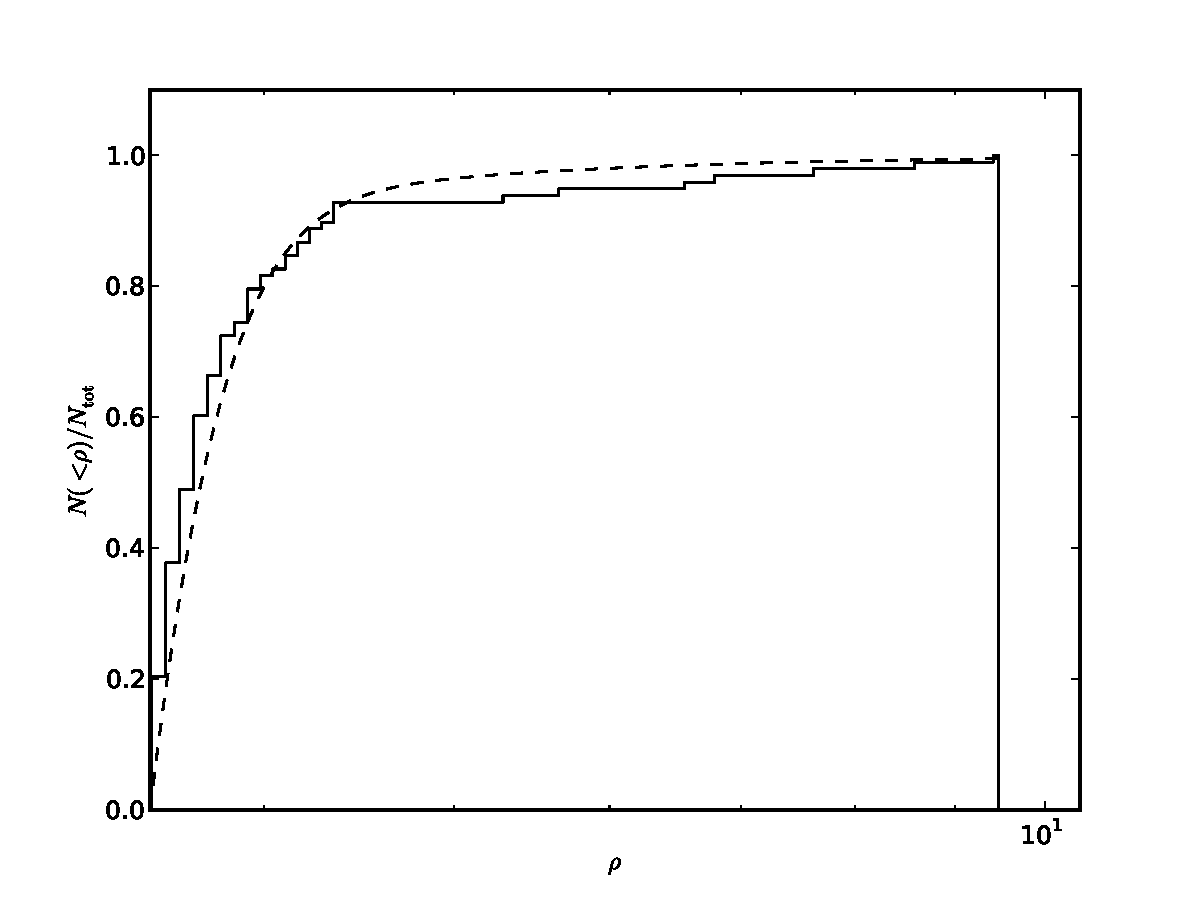
\includegraphics[width=\columnwidth]{data}
  \caption{\label{fig:analytic-data-cumulative} The cumulative
    distribution of the ranking statistics for the synthetic data used
    to test the formalism on the model from \S
    \ref{sec:analytic-GW-example}.  The solid line gives the
    cumulative distribution of the synthetic data; the dashed line
    gives the theoretical cumulative distribution for the models in
    Eqs.~\eqref{eq:analytic-background-rate} and
    \eqref{eq:analytic-foreground-rate} combined with $R_f = 10.4$ and
    $R_b = 95.1$. \ilya{[I think both axis labels should say $x$
        rather than $\rho$, since that's the ranking statistic ($\max
        \rho$).]}}
\end{figure}

In Figure \ref{fig:analytic-rate-recovery}, we show the marginalized
posterior densities for the foreground and background rates.  (Refer
to Eq.~\eqref{eq:rate-shape-posterior}.)  Figure
\ref{fig:analytic-rate-foreground-probs} shows the posterior
foreground probability for each event marginalized over all other
events' types and the foreground and background rates.

\ilya{[General comment on the text: I think we need to say a bit more
    about the figures and the interpretation of the results, instead
    of just relying on the reader to make the best of it.  For
    example, even though it may seem obvious to us, we should
    explicitly say that Fig.~2 shows that we succeed in recovering
    rates within the expected uncertainty envelope.  On Fig.~3, could
    say something obvious like point out that we cannot separate
    background from foreground for individual events, but that doesn't
    necessarily matter for rate measurements.  Now, one interesting
    question that Fig.~3 brings to mind is the following: if we only
    used "gold-plated" events (say, those with
    $p(x|fore)/p(x|back)>0.99$, how much worse / more uncertain would
    the rate estimation be?]}

\begin{figure}
  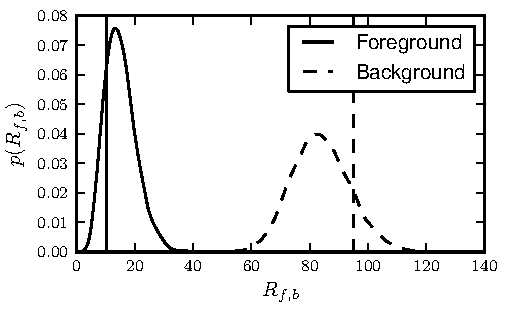
\includegraphics[width=\columnwidth]{rates}
  \caption{\label{fig:analytic-rate-recovery} The marginalized
    posterior densities for $R_f$ (solid line) and $R_b$ (dashed line)
    for the analytic model discussed in \S
    \ref{sec:analytic-GW-example}.  The vertical lines indicate the
    ``true'' values used to generate the synthetic data set.}
\end{figure}

\begin{figure}
  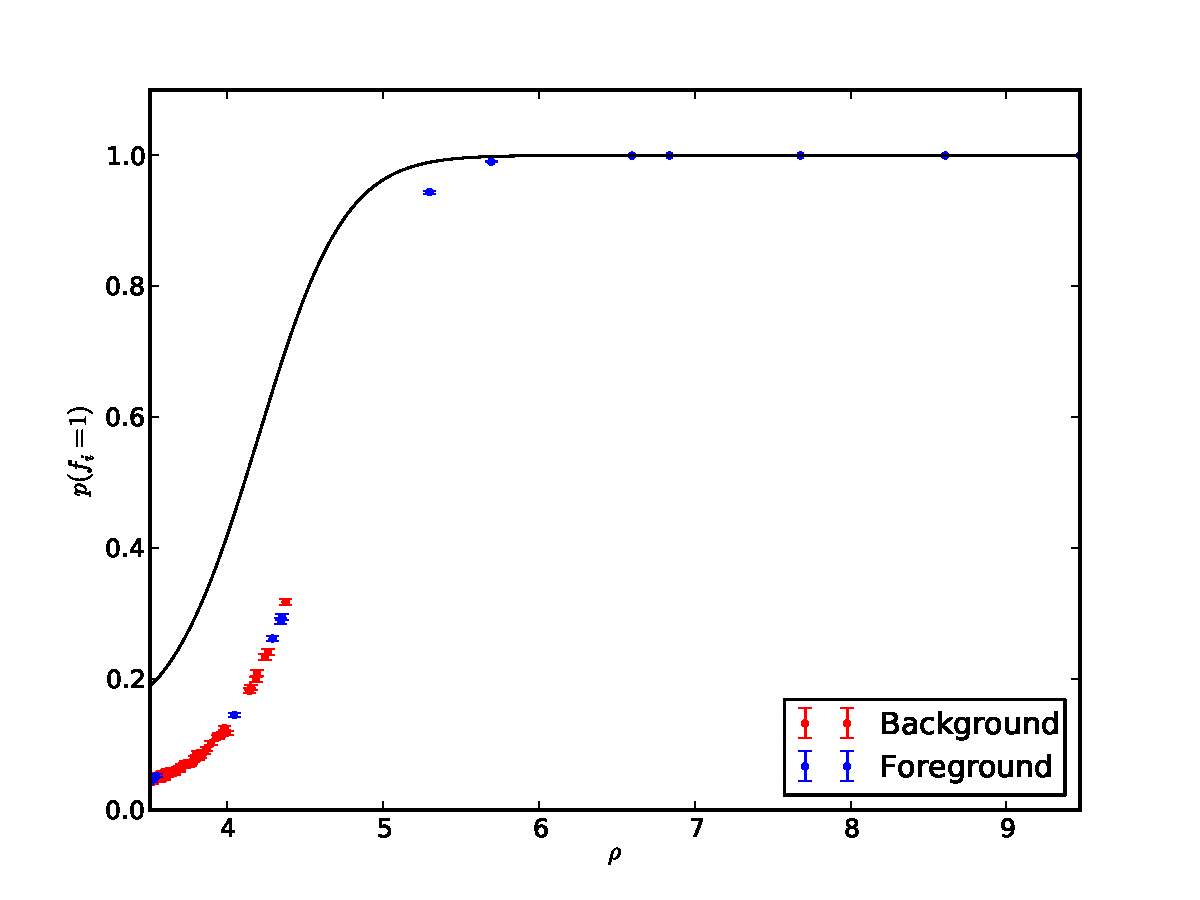
\includegraphics[width=\columnwidth]{pfore}
  \caption{\label{fig:analytic-rate-foreground-probs} Foreground
    probability for each event in the synthetic data set of \S
    \ref{sec:analytic-GW-example} marginalized over all other
    parameters.  True foreground events are in blue \ilya{(dark
      grey)}, background events in red \ilya{(light grey)}.  The solid
    line is the likelihood ratio
    $p(x|\mathrm{foreground})/p(x|\mathrm{background}) =
    \hat{f}(x)/\hat{b}(x)$ for this model \ilya{evaluated at the
      simulated parameters (?)}; this exceeds the marginalized
    foreground probability for many of the events because in this data
    set there are approximately nine times as many background events
    as foreground events. \ilya{[I'm not sure what the reader is meant
        to take away from the solid lines If there's something worth
        taking away, we should describe the message in the text.
        Otherwise, if it only confuses things, we should drop it.]}}
\end{figure}

\subsection{Gravitational Waves With Overlapping Templates}
\label{sec:gw-overlapping-template}

In \S \ref{sec:analytic-GW-example} we assumed that the overlap
between \ilya{different} templates in the template bank \ilya{was
  negligible}, so the SNRs \ilya{recovered by} different templates are
independent random variables.  In fact, template banks are not
constructed in this way \citep[e.g.,][]{Owen:1998dk,Ajith:2008},
%\citep{Caudill2011,Cannon2011}, 
because signals could fall in the gaps between the non-overlapping
templates.  We can model this effect by assuming that a template bank
of $N$ actual templates will behave as if it had $N_\mathrm{eff}$
\emph{independent} templates.  \ilya{Rather than pre-computing
  $N_\mathrm{eff}$,} we can fit for \ilya{it as a} shape parameter.
That is, we assume that \ilya{$\theta = \{N_\mathrm{eff}\}$} is a
shape parameter for the background cumulative distribution:
\begin{equation}
  \hat{B}\left(x, N_\mathrm{eff}\right) = \frac{\left( 1 + \erf\left( \frac{x}{2} \right)
    \right)^{N_\mathrm{eff}} - \left( 1 + \erf\left( \frac{\xmin}{2} \right)
    \right)^{N_\mathrm{eff}}}{2^{N_\mathrm{eff}} - \left( 1 + \erf\left( \frac{\xmin}{2} \right)
    \right)^{N_\mathrm{eff}} }.
\end{equation}

Results from such an analysis appear in Figures \ref{fig:rates-nt} and
\ref{fig:ntemplates}.  We use the same parameters and data set as in
\S \ref{sec:analytic-GW-example}, with $R_f = 10.4$, $R_b = 95.1$, and
$N_\mathrm{eff} = 1000$, but now allow $N_\mathrm{eff}$ to be a
parameter of the background distribution, with a flat prior.  Both the
rates and the number of effective templates are recovered without
significant loss of accuracy relative to the fixed $N_\mathrm{eff}$
situation in \S \ref{sec:analytic-GW-example}.

\ilya{[Again, I think we need to explicitly compare this method with
    two alternatives.  Alternative one is the loudest event statistic.
    Alternative two is just counting gold-plated events, and dividing
    the volume in which we are sensitive to them by their number.  In
    principle, alternative one should be suboptimal when the number of
    events is more than 0 or 1, while alternative two should be OK
    when the number of events is large, but error-prone otherwise.
    But if we want people to use this technique, we have to defend the
    point that there is a regime where it is clearly superior (and say
    what that regime is).]}

\begin{figure}
  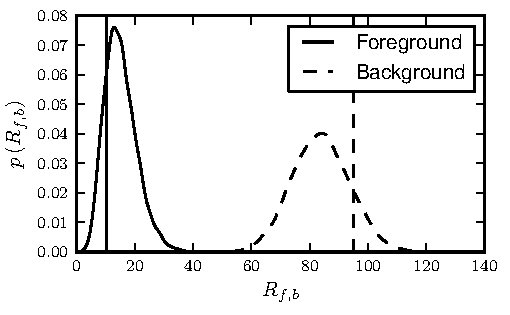
\includegraphics[width=\columnwidth]{rates-nt}
  \caption{\label{fig:rates-nt} The foreground (solid lines) and
    background (dashed lines) rate posterior, marginalized over all
    flags and the $N_\mathrm{eff}$ parameter, for the gravitational
    wave template detection scenario with overlapping templates
    discussed in \S \ref{sec:gw-overlapping-template}.  The true
    values of the rates, $R_f = 10.4$ and $R_b=95.1$, are indicated
    with vertical lines.  The distributions are not significantly
    wider than those of Figure \ref{fig:analytic-rate-recovery}, in
    spite of the extra parameter.  \ilya{[$R_f$ seems to be more of an
        outlier than before; why was there a significant shift, given
        that $N_\mathrm{eff}$ seems fairly spot on?]}}
\end{figure}

\begin{figure}
  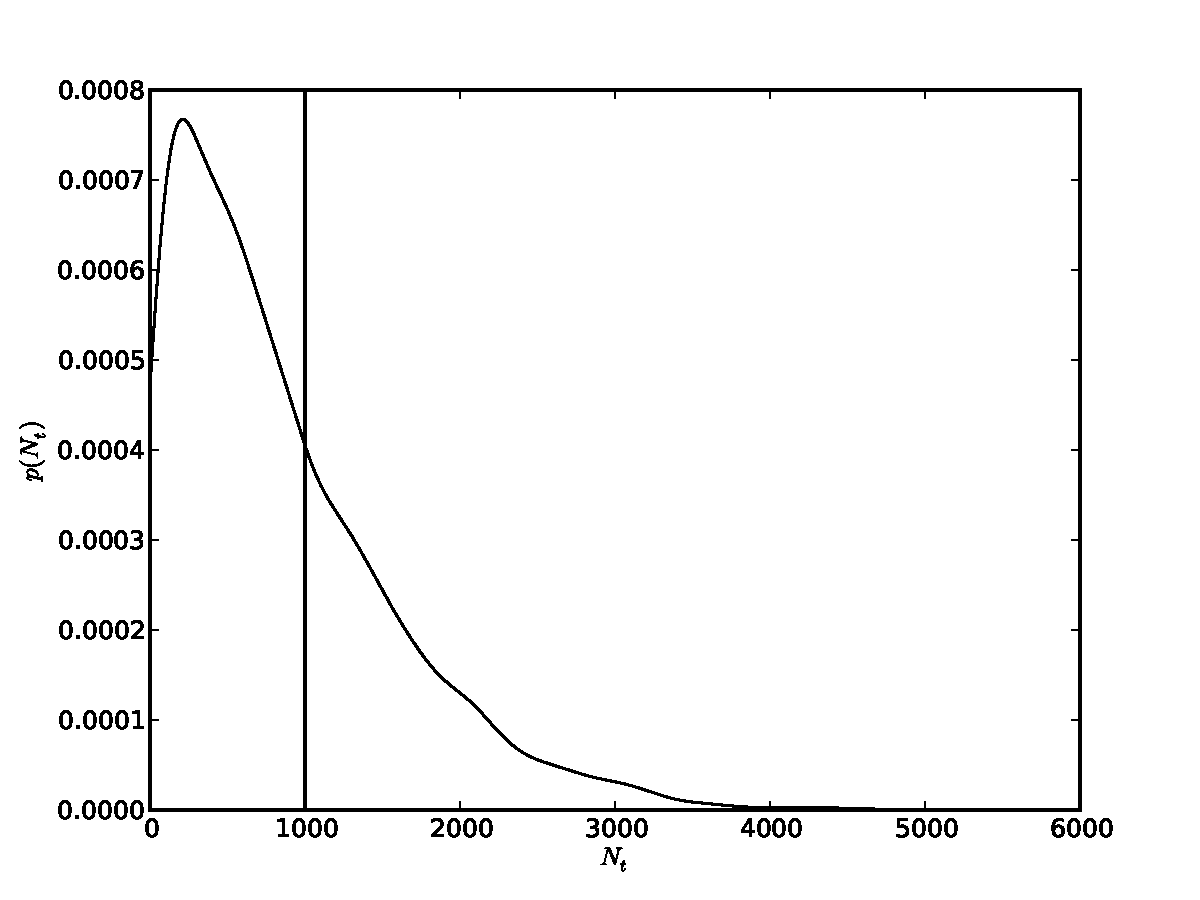
\includegraphics[width=\columnwidth]{ntemplates}
  \caption{\label{fig:ntemplates} The posterior on the number of
    effective templates, $N_\mathrm{eff}$, for the model and data
    discussed in \S \ref{sec:gw-overlapping-template}, marginalized
    over all state flags and rates.  The true value, $N_\mathrm{eff} =
    1000$, is indicated by the vertical line.}
\end{figure}

\subsection{Star Cluster Parameters With Background Contamination}
\label{sec:star-cluster}

Our final example concerns fitting for the location and shape
parameters of a cluster of stars observed on top of a stellar
background with a density gradient.  We assume that a star cluster has
a Plummer surface-density profile \citep{Plummer1911,Aarseth1974},
\begin{equation}
  \label{eq:plummer-surface-density}
  \hat{f}(\vec{x}, \theta) = \frac{1}{\pi r_0^2 \left( 1 + \frac{\left|
          \vec{x} - \vec{x}_0 \right|^2}{r_0^2} \right)^2},
\end{equation}
where $\vec{x}_0$ is the location on the sky of the center of the
cluster, and $r_0$ is a radial scale parameter.  We assume a square
observational domain\footnote{The observational domain is not
  infinite, so the normalization of the cluster density in
  Eq.~\eqref{eq:plummer-surface-density} is not quite correct.  In our
  modeling we properly take this into account, but for simplicity here
  we ignore it.}, $\vec{x} \in [0,1]^2$, and a background that has a
density gradient at an arbitrary orientation with respect to the
observational axes:
\begin{equation}
  \hat{b}\left(\vec{x}, \theta\right) = 1 + \vec{\gamma} \cdot \left( \vec{x}
    - \vec{x}_{1/2} \right),
\end{equation}
where $\vec{\gamma}$ is the gradient, and $\vec{x}_{1/2} = [1/2, 1/2]$
is the centroid of the observational domain.  \ilya{[I think that if
    the domain is finite, the previous equation is only normalized for
    all $\vec{\gamma}$ if $\vec{x}_{1/2}$ is in the center of a
    symmetric domain (as it happens to be in this case).]}  We use
assume a gradient for the background of $\vec{\gamma} = [-0.5, 0.5]$.
\ilya{[I find it a bit confusing to use the word "assume" for both the
    model and for the specific parameters injected into the simulation
    (but then being fit for, so their values are not "assumed" in the
    recovery).  Maybe "assume" for the model, and "simulate" for the
    parameter values to be fit?]}  We assume that the total number of
background stars, $R_b = 10000$, exceeds by a factor of ten the total
number of cluster stars, $R_f = 1000$.  \ilya{[But the cluster has
    only $\sim 0.01$ of the total area, so it's over-dense by a factor
    of $10$ or more.  Fig.~6 shows a very bright spot where the
    cluster is, which sort of makes the problem look too simple for
    the chosen parameters...]}  We choose a true cluster center
$\vec{x}_0 = \vec{x}_{1/2}$, and a radial scale parameter of $r_0 =
0.1$.  In all, the shape parameters for the true distributions are
\begin{equation}
\label{eq:true-cluster-parameters}
\theta_0 \equiv \left\{ x_0, y_0, r_0, \gamma_x, \gamma_y \right\} =
\left\{ \frac{1}{2}, \frac{1}{2}, \frac{1}{10}, -\frac{1}{2},
  \frac{1}{2} \right\}.
\end{equation}
Figure \ref{fig:sky-density} shows the density on the sky due to the
cluster foreground and the background with these parameters.  We drew
a synthetic data set from this density according to the corresponding
inhomogeneous Poisson process.

\begin{figure}
  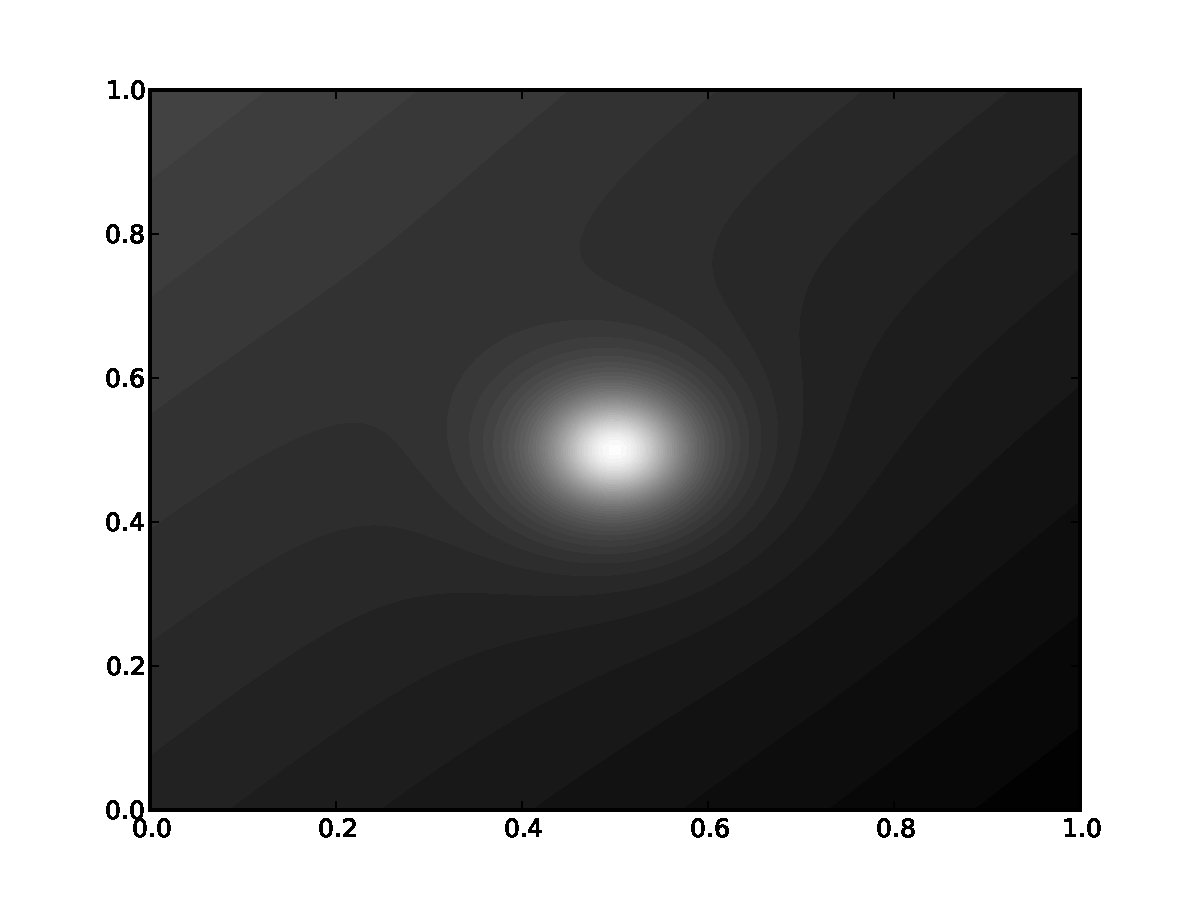
\includegraphics[width=\columnwidth]{sky-density}
  \caption{\label{fig:sky-density} The density contours on the sky of
    the forergound cluster and background discussed in \S
    \ref{sec:star-cluster}, with true parameters given in
    Eq.~\eqref{eq:true-cluster-parameters}.  There are a factor of 10
    more stars (10000) in the background than in the cluster (1000),
    but the peak density for the cluster is much higher.  \ilya{[It
        seems too obvious that where the cluster is by eye, and
        probably fairly straightforward to compute the number of
        "excess" stars there...  Reader might ask why we need
        something so complicated when the answer is seems so obvious
        and a "frequentist" approach would seem to do here.]}}
\end{figure}

To analyze our synthetic data set, we analytically marginalized over
the state flags, using the likelihood in Eq.~\eqref{eq:rate-shape-posterior}.
\ilya{[I think it would be kind to the reader to be more explicit
    about the connection with the formalism in Section II.  What are
    the "events"?  What is the ranking statistic $x$?  What are the
    flags (which aren't in $\mathbb{R}$?)?]}  We did this to take
advantage of the \textit{emcee} sampler of \citet{ForemanMackey2012},
which requires all parameters to be in $\mathbb{R}$.  We applied a
prior on the shape parameters that is flat in $\vec{x}_0$ and
$\vec{\gamma}$, and the Jeffreys prior on $r_0$,
\begin{equation}
  p\left( r_0 \right) = \frac{\sqrt{R_f}}{r_0}.
\end{equation}
\ilya{[Why is this the Jeffreys prior (BTW, it's Jeffreys, or perhaps
    Jeffreys', but definitely not Jeffrey's ;) )?  It's not obvious
    why the prior on $r_0$ should depend on $R_f$?]}  (Note that this
factor of $\sqrt{R_f}$ cancels with the Jeffreys prior on the rate,
$1/\sqrt{R_f}$; we have verified that the priors on these parameters
are irrelevant to our results, as would be expected from the
measurement of $\sim 1000$ foreground stars.)

Figure \ref{fig:sky-loc} shows the posterior for the location
parameters, $\vec{x}_0$; the center of the cluster is localized to
within a few percent of its scale.  Figure \ref{fig:cluster-number}
shows the posteriors inferred on the cluster and background numbers,
$R_f$ and $R_b$, and Figure \ref{fig:cluster-scale} shows the
posterior for the cluster's scale parameter.  In spite of the
significant background, the cluster scale and total number are
accurately recovered by our analysis.

\begin{figure}
  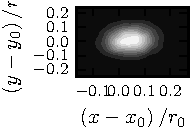
\includegraphics[width=\columnwidth]{sky_location}
  \caption{\label{fig:sky-loc} Contours of the posterior probability
    distribution for the center of the cluster, $\vec{x}_0$, in the
    example from \S~\ref{sec:star-cluster}.  The center $(x,y) =
    \left(x_0, y_0\right)$ is determined to within a few percent of
    the structural radius of the cluster, $r_0$ (see
    Eq.~\eqref{eq:true-cluster-parameters}). \ilya{[Given the cluster
        size of 0.1, it seems a bit surprising that the center is off
        by $\sim 0.05$...]}}
\end{figure}

\begin{figure}
  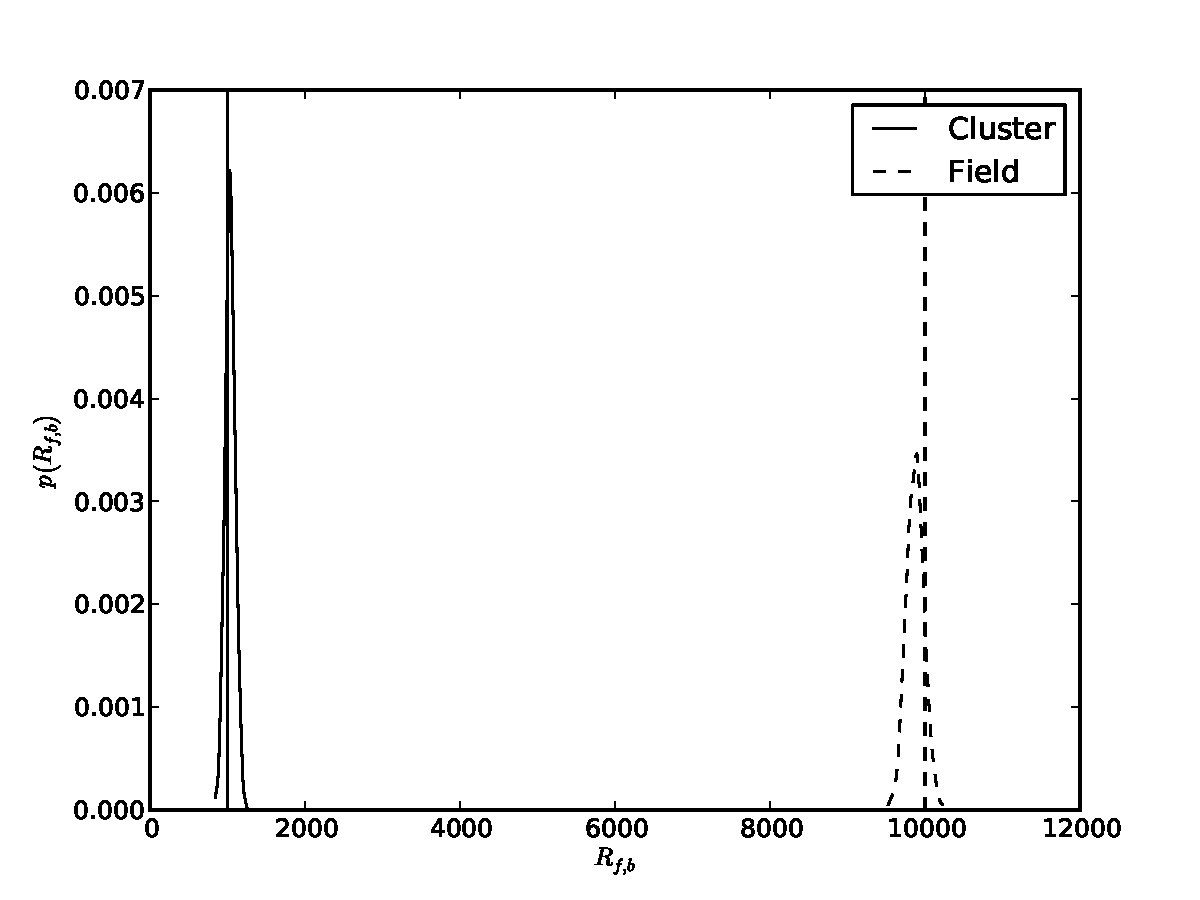
\includegraphics[width=\columnwidth]{numbers}
  \caption{\label{fig:cluster-number} Posterior densities for the
    number of stars in the cluster ($R_f$) and in the field ($R_b$) in
    the example from \S~\ref{sec:star-cluster}.  Vertical lines
    indicate the true values (see
    Eq.~\eqref{eq:true-cluster-parameters}). }
\end{figure}

\begin{figure}
  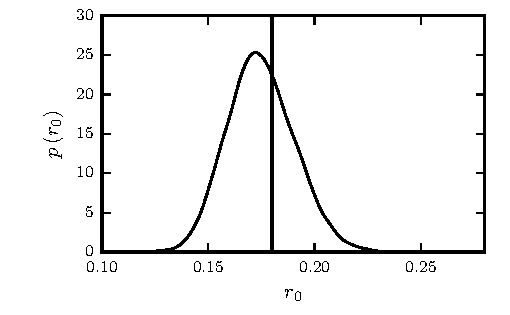
\includegraphics[width=\columnwidth]{scale}
  \caption{\label{fig:cluster-scale} Posterior density for the scale
    parameter for the cluster, $r_0$, from the example in
    \S~\ref{sec:star-cluster}.  The true value is indicated by the
    vertical line (see Eq.~\ref{eq:true-cluster-parameters}).
    \ilya{[Perhaps combine Figs.~8 and 9 (put an extra scale for $r_0$
        at the top of 8?]} }
\end{figure}

\section{Conclusion}

Separating classes of events

Comments on background probability estimation --  Cannon et al. in prep.

Relevance (vs. loudest statistic, or frequentist approach using only
gold-plated events)

\begin{acknowledgments}
  We thank Kipp Cannon, Chad Hanna, Drew Keppel, and Richard
  O'Shaughnessy for discussions and suggestions about this manuscript.
\end{acknowledgments}

%%%%%%%%%%%%%%%%%%%% Bibliography 
\bibliographystyle{apsrev4-1}
\bibliography{many}

\end{document}
